\let\negmedspace\undefined
\let\negthickspace\undefined
\documentclass[journal]{IEEEtran}
\usepackage[a5paper, margin=10mm, onecolumn]{geometry}
\usepackage{lmodern} % Ensure lmodern is loaded for pdflatex
\usepackage{tfrupee} % Include tfrupee package

\setlength{\headheight}{1cm} % Set the height of the header box
\setlength{\headsep}{0mm}     % Set the distance between the header box and the top of the text

\usepackage{gvv-book}
\usepackage{gvv}
\usepackage{cite}
\usepackage{amsmath,amssymb,amsfonts,amsthm}
\usepackage{algorithmic}
\usepackage{graphicx}
\usepackage{textcomp}
\usepackage{xcolor}
\usepackage{txfonts}
\usepackage{listings}
\usepackage{enumitem}
\usepackage{mathtools}
\usepackage{gensymb}
\usepackage{comment}
\usepackage[breaklinks=true]{hyperref}
\usepackage{tkz-euclide} 
\usepackage{listings}
\usepackage{gvv}                                        
\def\inputGnumericTable{}                                 
\usepackage[latin1]{inputenc}                                
\usepackage{color}                                            
\usepackage{array}                                            
\usepackage{longtable}                                       
\usepackage{calc}                                             
\usepackage{multirow}                                         
\usepackage{hhline}                                           
\usepackage{ifthen}                                           
\usepackage{lscape}
\begin{document}

\bibliographystyle{IEEEtran}
\vspace{3cm}

\title{12.8.3.11}
\author{EE24BTECH11024 - G. Abhimanyu Koushik}
% \maketitle
% \newpage
% \bigskip
{\let\newpage\relax\maketitle}
\textbf{Question:}
Using the method of integration find the area bounded by the curve $\abs{x} + \abs{y} = 1$
\solution\newline
Theoretical Solution:\newline
The curve $\abs{x} + \abs{y} = 1$ consists of 4 lines
\begin{align}
	x+y&=1\\
	-x+y&=1\\
	x-y&=1\\
	-x-y&=1
\end{align}
Solving the line equations\newline
Let the line equations be $\vec{x} = \vec{h}_1 + \kappa_1\vec{m}_1$ and $\vec{x} = \vec{h}_2 + \kappa_2\vec{m}_2$ then
\begin{align}
	\vec{h}_2 + \kappa_2\vec{m}_2 &= \vec{h}_1 + \kappa_1\vec{m}_1\\
	\vec{h}_1 - \vec{h}_2 &=  \kappa_2\vec{m}_2 - \kappa_1\vec{m}_1\\
	\vec{h}_1 - \vec{h}_2 &= \myvec{\vec{m}_2 & -\vec{m_1}}\myvec{\kappa_2\\\kappa_1}
\end{align}
Solving the equation using row reduction gives the value of $\kappa_1$ and $\kappa_2$ which can be subsituted in line equation to get the point\newline
For the given lines, the values of $\vec{m}$ and $\vec{h}$ are
\begin{align}
	\vec{m}_1 = \myvec{-1\\1}\\
	\vec{m}_2 = \myvec{1\\1}\\
	\vec{m}_3 = \myvec{1\\1}\\
	\vec{m}_4 = \myvec{-1\\1}\\
	\vec{h}_1 = \myvec{1\\0}\\
	\vec{h}_2 = \myvec{0\\1}\\
	\vec{h}_3 = \myvec{0\\-1}\\
	\vec{h}_4 = \myvec{-1\\0}
\end{align}
The matrix equations we get for lines \brak{1,2} is
\begin{align}
	\myvec{1\\-1} = \myvec{1 & 1\\1 & -1}\myvec{\kappa_2\\\kappa_1}
\end{align}
The augmented matrix for this will be
\begin{align}
  \myvec{1 & 1 & 1\\1 & -1 & -1}  &\xleftrightarrow[]{R_2 \leftarrow {R_1-R_2}}\myvec{1 & 1 & 1 \\0 & 2 & 2}\\
  &\xleftrightarrow[]{R_1 \leftarrow {R_1-\frac{R_2}{2}}}\myvec{1 & 0 & 0 \\0 & 2 & 2}\\
  &\xleftrightarrow[]{R_2 \leftarrow {\frac{R_2}{2}}}\myvec{1 & 0 & 0 \\0 & 1 & 1}\\
  \kappa_1 &= 1
\end{align}
Substituting $\kappa_1$ in line equation gives first intersection point to be
\begin{align}
	\vec{x}_1 = \myvec{1\\0} + \myvec{-1\\1}\\
	\vec{x}_1 = \myvec{0\\1}
\end{align}
Similarly the other intersection points are \brak{1,0}, \brak{-1,0}, and \brak{0,-1} forming a square. To find the area we can integrate $x+y=1$ from $x=0$ to $x=1$ and then multiply the area by 4 to get the total area   
\begin{align}
	A_0 &= \int_{0}^{1}\brak{1-x}dx\\
	A_0 &= \brak{x-\frac{x^2}{2}}\Big|_0^1\\
	A_0 &= \frac{1}{2}\\
	A &= 4A_0\\
	A &= 2
\end{align}

Computational Solution:\newline

Taking trapezoid shaped strips of small area and adding them all up. Say we have to find the area of $y\brak{x}$ from $x=x_0$ to $x=x_n$, discretize points on the $x$ axis $x_0, x_1, x_2, \dots, x_n$ such that they are equally spaced with step-size $h$. \newline
Sum of all trapezoidal areas is given by,
\begin{align}
  A&=\frac{1}{2}h\brak{y\brak{x_1}+y\brak{x_0}}+ \frac{1}{2}h\brak{y\brak{x_2}+y\brak{x_1}}+\dots+\frac{1}{2}h\brak{y\brak{x_n}+y\brak{x_{n-1}}}\\
  &=h\sbrak{\frac{1}{2}\brak{y\brak{x_0}+y\brak{x_n}}+ y\brak{x_1}+\dots+y\brak{x_{n-1}}}
\end{align}
Let $A\brak{x_n}$ be the area enclosed by the curve $y\brak{x}$ from $x=x_0$ to $x=x_n$, $\brak{x_0, x_1, \dots x_n}$ be equidistant points with step-size $h$.
\begin{align}
  A\brak{x_n+h}=A\brak{x_n}+\frac{1}{2}h\brak{y\brak{x_n+h}+y\brak{x_n}}
\end{align}
We can repeat this till we get required area.\newline
Discretizing the steps, making $A\brak{x_n}=A_n, y\brak{x_n}=y_n$ we get,
\begin{align}
 A_{n+1}=A_n+\frac{1}{2}h\brak{y_{n+1}+y_n}
\end{align}
We can write $y_{n+1}$ in terms of $y_n$ using first principle of derivative. $y_{n+1}=y_n+hy^{\prime}_n$
\begin{align}
  A_{n+1}&=A_n+\frac{1}{2}h\brak{\brak{y_{n}+hy^{\prime}_n}+y_n}\\
  A_{n+1}&=A_n+\frac{1}{2}h\brak{2y_n+hy^{\prime}_n}\\
  A_{n+1}&=A_n+hy_n+\frac{1}{2}h^2y^{\prime}_n\\
  x_{n+1}&=x_n+h
\end{align}

In the given question, $y_n=1 - x_n$ and $y^{\prime}_n=-1$\newline
General Difference Equation will be given by,
\begin{align}
  A_{n+1}&=A_n+hy_n+\frac{1}{2}h^2y^{\prime}_n\\
  A_{n+1}&=A_n+h\brak{1-x_n}+\frac{1}{2}h^2\brak{-1}\\
  A_{n+1}&=A_n -hx_n+\brak{h-\frac{h^2}{2}}\\
  x_{n+1}&=x_n+h
\end{align}
Iterating till we reach $x_n=1$ will return required area. Note, Area obtained is to be multiplied by $4$ as the calculated area only accounts for one quater of the graph.\newline
The calculated area is $4\times 0.5$ which is $2$.
\begin{figure}[h!]
   \centering
   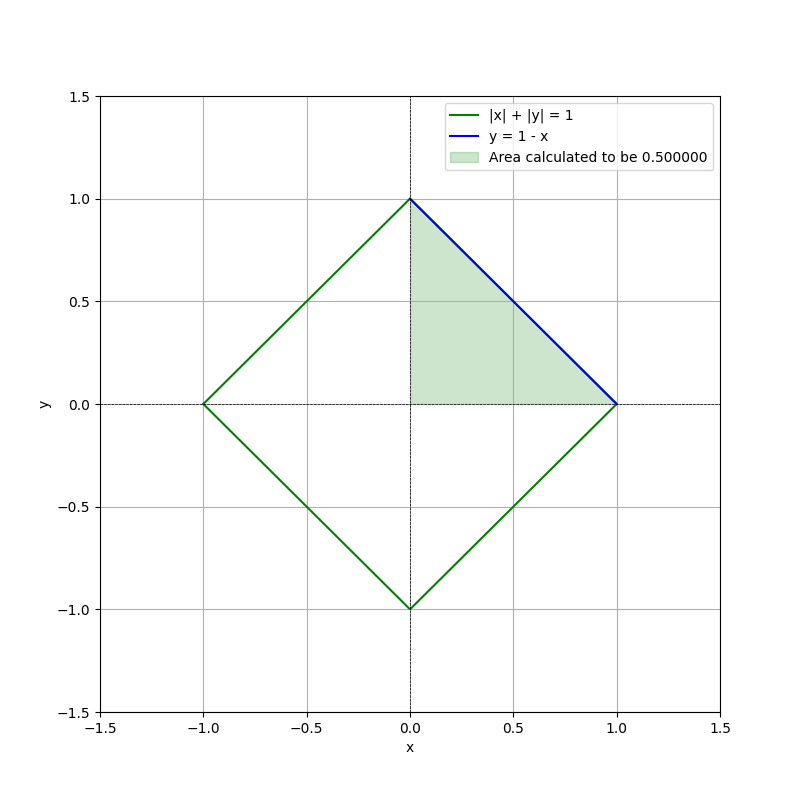
\includegraphics[width=1\columnwidth]{figs/fig.png}
   \caption{Graph of the parabola $\abs{x}+\abs{y} = 1$ and $x+y=1$ and the area of which the integral is calculated}
   \label{stemplot}
\end{figure}
\end{document}
